\section{Verwendete Technologien}

\subsection{RIOT}
RIOT ist ein neues Betriebssytem für das Internet of Things (IoT).
Es ist ein teilweise POSIX-konformes System, das auf mehreren Hardwareplattformen lauffähig ist.
Die Programmierung gestaltet sich sehr bequem, da einfach in C oder C++ programmiert werden kann, unter Verwendung von Standardwerkzeugen wie gcc und gdb.
Es zeichnet sich durch eine minimale Hardwareabhängigkeit aus ist dementsprechend einfach zu portieren.

RIOT ist außerordentlich resourcenschonend und ermöglicht dabei eine maximale Energieeffizienz, was vor allen Dingen für eingebettete Systeme entscheidend ist.
Zusätzlich ist das System Multithreading-fähig und unterstützt viele für das IoT relevante Netzwerkprotokolle. Dazu kommt eine Echtzeitfähigkeit.

\subsubsection{native port}
\label{section:native_port}
Der native port ist eine Version von RIOT, welche als regulärer Prozess innerhalb eines Linux-Systemes ausgeführt werden kann.
Vergleichbar ist dies mit Lösungen wie User Mode Linux.
Dies ermöglicht das Testen und Implementieren von hardwareunabhängigen Funktionen innerhalb von RIOT ohne auf einer eingebetteten Plattform jedes mal flashen zu müssen.
Ferner können alle Funktionen des Wirtsystemes verwenden werden.
Insbesondere bedeutet dies auch, dass der Arbeitsspeicher des Wirtsystemes im vollen Maße verwendet werden kann.

\subsubsection{Treiberarchitektur}
Um die hohe Portabilität von RIOT zu gewährleisten, sind alle Treiber prizipiell in einen hardwareabhängigen und einen hardwareunabhängigen Teil getrennt.
Dies hat zur Folge, dass bei der Portierung von RIOT auf eine neue Plattform der hardwareabhängige Teil angepasst werden muss.

\subsection{USB}
Der \textbf{U}niversal \textbf{S}erial \textbf{B}us ist ein serieller Bus, der die Kommunikation von Peripheriegeräten mit dem Computer ermöglicht.
Die Kommunikation läuft immer zwischen zwei Endpunkten ab.
Ein Endpunkt ist eine Art Unteradresse in einem USB-Gerät.
Viele Geräte besitzen Unterfunktionen, denen dann jeweils ein Endpunkt zugeordnet ist.
USB kennt verschiedene Übertragungsmodi:

\paragraph{Synchroner Transfer}
Beim synchronen Transfer (auch Kontrolltransfer genannt) werden durch eine bidirektionale Pipe kurze Datenpakete zwischen zwei Endpunkten hin und her geschickt.
Diese Art des Datentransfers ist speziell für die Konfiguration von Geräten entworfen worden.

\paragraph{Asynchroner Transfer}
Der asynchronen Transfer kann dadurch charaterisiert werden, dass die Antwortpakete vom Gerät zu beliebigen Zeitpunkt beim Sender eintreffen.
Die Verarbeitung der übertragenen Daten muss folglicherweise auch asynchron erfolgen.
Die Übertragung aynchroner Pakete ist generell mit einer CRC16-Prüfsumme gesichert.
Dies bedeutet jedoch nicht, dass bei einem fehlerhaften Transfer automatisch eine Übertragungswiederholung durchgeführt wird, sondern dass erkannt werden kann, ob ein Paket fehlerhaft ist.
Beim asynchronen Transfer unterscheidet man wiederum in folgende drei Submodi:

\paragraph*{Bulk-Transfer}
Der Bulk-Transfer ist vor allen Dingen für die Übertragung von großen Datenmengen gedacht.
Da diese oftmals nicht zeitkritisch sind, wird diese Form des Transfers niedrig priorisiert und erst durchgeführt, wenn isochrone Transfers und Interrupt-Transfers abgeschlossen sind.

\subparagraph{Interrupt-Transfer}
Interrupt-Transfers sind dafür da, um kleine Datenmengen schnell und unter Umständen häufig zu übertragen, daher wird diese Form des Transfers hauptsächlich für Eingabegeräte wie Maus und Tastatur verwendet.

\subparagraph{Isochroner Transfer}
Die Form des Transfers garantiert eine bestimmte Datenrate zwischen zwei Endpunkten.
Bei der Initialisierung einer solchen Verbindung muss die gewünschte Datenrate explizit auf dem USB-Hostcontroller reserviert werden. (vgl. \emph{Alternate Setting})
Zur Steigerung der Datenrate ist es möglich, mehrere isochrone Transfers parallel zwischen mehreren Endpunkten ablaufen zu lassen.
Isochroner Transfer läuft im Grunde genommen so ab, dass vorbereitete, leere Datenpakete verschickt werden, die dann auf der Geräteseite mit den zu übertragenden Daten gefüllt werden und als Antwortpakete zurückgesendet werden.

\subsection{USB-Video-Grabber}
Das Kernstück des Projektes war der \emph{EasyCAP}-USB-Video-Grabber.
Hierbei handelt es sich um einen günstigen Grabber, der einen S-Video-Eingang, einen Composite-Videoeingang und einen Zweikanal-Audioeingang besitzt.
Auf dem Grabber finden sich im Wesentlichen zwei Chips.
\begin{figure}[h]
 \centering
 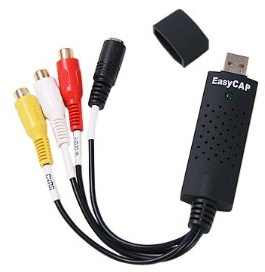
\includegraphics[width=.5\textwidth]{grabber}
 \caption{Der \emph{EasyCAP}-USB-Grabber}
\end{figure}

\subsubsection{Videochip \saa}
Der von \emph{Philips Semiconductors} entwicklte \saa{} ist ein 9-Bit-Videoprozessor, der mehrere Eingangssignale verarbeiten und dabei umfangreiche Bildanpassungen wie Helligkeits- und Kontrastanpassung, Farbkorrektur und Rauschreduzierung in Echtzeit durchführen kann.
Fener zeichnet er sich durch eine äußerst kompakte Baugröße und einen niedrigen Energiebedarf aus.
% TODO Quellenangabe: http://pvr.sourceforge.net/SAA7113H_1.pdf

\subsubsection{USB-Gateway-Chip \stk}
Der zweite verbaute Chip ist der von \emph{Syntek Semiconductor} entwickelte USB-Gateway-Chip \stk.
Jener ist zum einen mit dem \saa{} über den von \emph{Philips Semiconductors} entwickelten seriellen Datenbus \iic{} (Inter-Integrated Circuit) und zum anderen über USB~2.0 mit dem Computer verbunden.

\paragraph{\iic}
\iic{} ist ein serieller Datenbus, der entwickelt wurde, um eine einfache, standardisierte Möglichkeit zu besitzen, um zwischen verschiedenen Mikrochips kommunizieren zu können.
Die Kommunikation beschränkt sich hierbei auf Steuerinformationen.
Der Bus ist wie auch USB als Master-Slave-Bus konzipiert, wobei es immer der Master ist, der den Datentransfer beginnt.
In unserem Falle stellt der \stk{} den Master und der \saa{} den Slave dar.

\subsubsection{Zusammenspiel der Chips}
\label{section:zusammenspiel}
Der Computer oder allgemeiner, das Hostsystem kommuniziert immer nur mit dem \stk, nie jedoch mit dem \saa{} direkt.
Sämtliche Steuerinformationen, in der Regel die Manipulation von Registern, die den \stk{} betreffen, werden in USB-Kontrollnachrichten verpackt und an den \stk{} mittels synchronem Transfer gesendet.
Ist es notwendig, Steuerinformationen an den \saa{} zu senden, läuft die Kommunikation folglicherweise über den \stk.
In diesem Falle müssen auch USB-Kontrollnachrichten an den \stk{} gesendet werden, der bei bestimmten Werten in jenen Nachrichten die nötigen Steuerinformationen über \iic{} an den \saa{} weiterleitet.
Die eigentliche Übertragung der Videoinformationen von der Videoquelle durch den \saa{} und dann über den \stk{} zum Hostsystem erfolgt nicht über \iic, da jenes Protokoll mit einer maximalen Datenrate von 3,4\,MBit/s viel zu langsam wäre.
Stattdessen existiert neben dem \iic-Bus eine weitere, 8\,Bit breite Datenverbindung, der \emph{VPO}-Bus.
\begin{figure}[h]
 \centering
 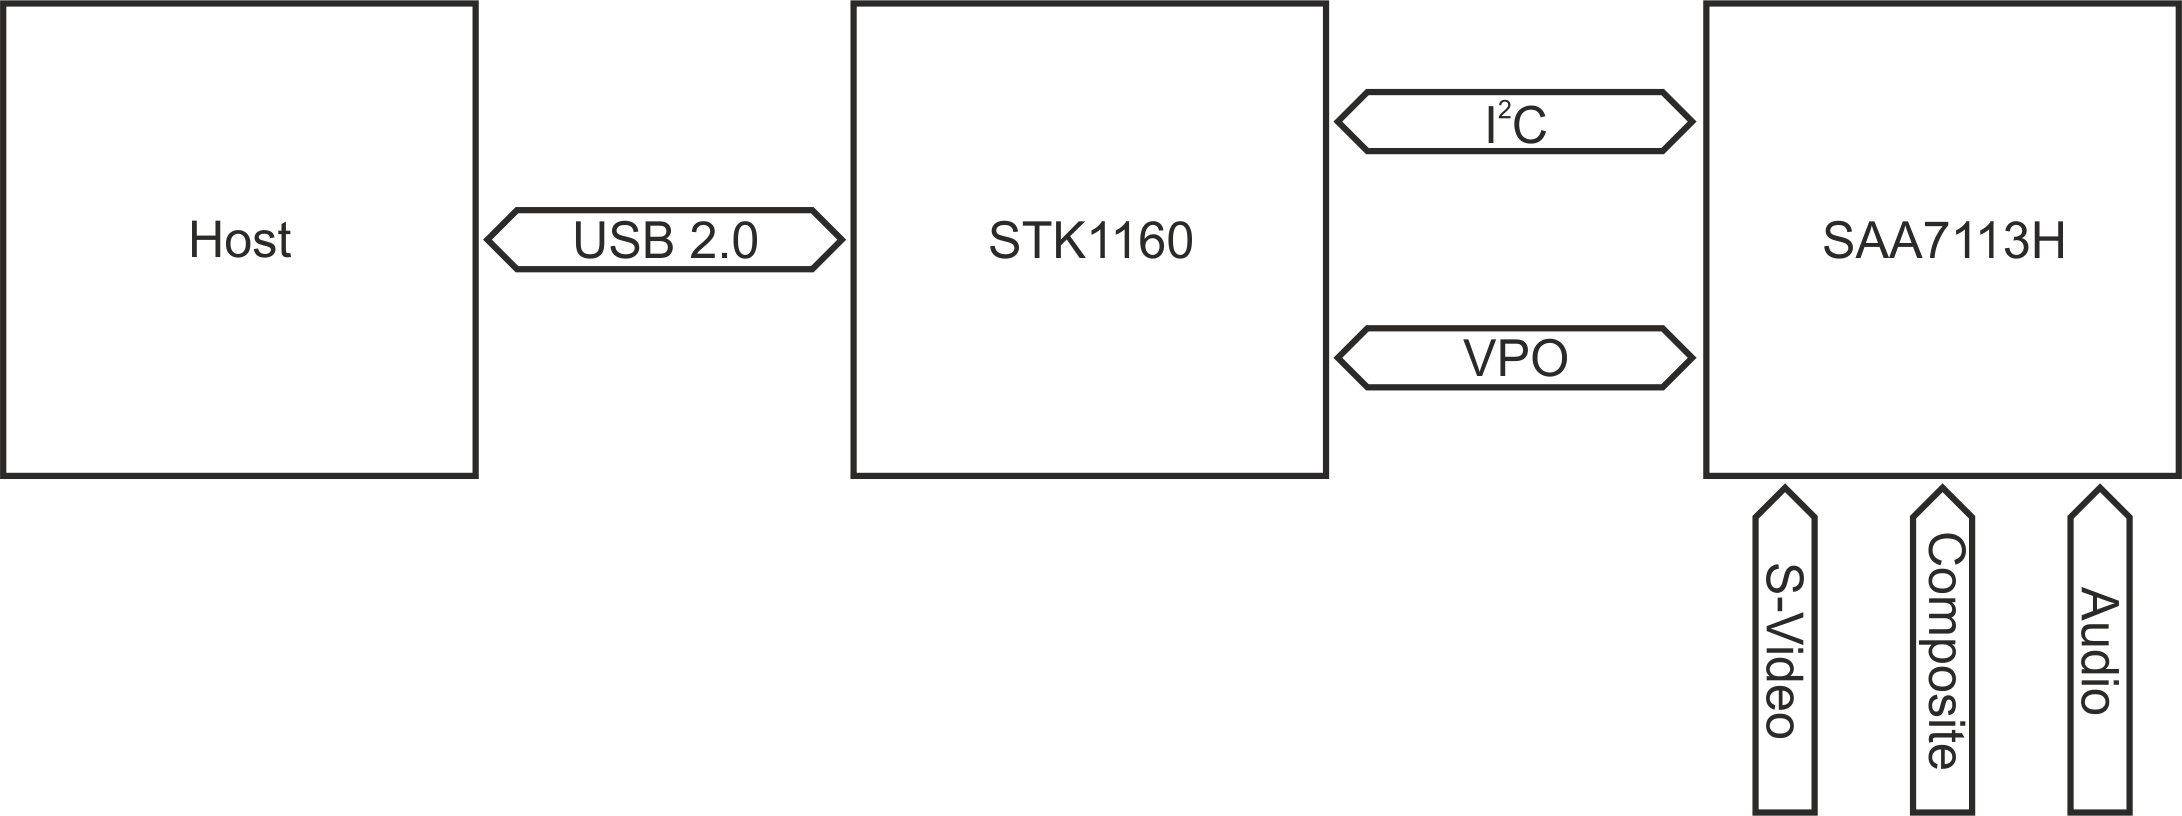
\includegraphics[width=\textwidth]{blockschaltbild}
 \caption{Blockschaltbild des \emph{EasyCAP}-USB-Grabbers}
\end{figure}

\subsubsection{Übertragung der Videodaten}
Wenn die Videoübertragung beginnen soll, wird ein Register im \saa{} gesetzt.
Die Videodaten werden dann fortlaufend über den \emph{VPO}-Bus in einen Puffer im \stk{} abgelegt.
Werden die Daten vom Hostsystem nicht über isochronen USB-Datentransfer "`abgeholt"', werden sie im Puffer fortlaufend überschrieben.
Liegt jedoch eine leere isochrone USB-Nachricht vor, liest der \stk{} die Videodaten aus dem Puffer aus und schreibt sie in die Nachricht und schickt jene über den USB-Bus zum Hostsystem zurück.